\documentclass{assignmeownt}

\usepackage{graphicx}
\usepackage{pdflscape}
\usepackage{lscape}
\usepackage{svg}
\graphicspath{ {./images/} }

\coursenumber{MTL782}
\coursetitle{Data Mining}
\doctitle{Assignment 1}
\docauthor{Saket Kandoi 2021MT60265 \\ Navneet Raj 2021MT10240 \\ Aditya Thomas 2021MT60944}

%%%%%%%%%%%%%%%%%%%%%%%%%%%%%%%%%%%%%%%%%%%%%%%%%%%%%%%%%%%%%%%%%
%%%             Landscape Environment                         %%%
%%%        (Must load etoolbox package before)                %%%
%%%    And use /savegeometry before the using landscape page  %%%
%%%      and use /loadgeometry after the landscape page       %%%
%%%%%%%%%%%%%%%%%%%%%%%%%%%%%%%%%%%%%%%%%%%%%%%%%%%%%%%%%%%%%%%%%

\makeatletter
 \def\ifGm@preamble#1{\@firstofone}
  \appto\restoregeometry{%
     \pdfpagewidth=\paperwidth
     \pdfpageheight=\paperheight}
 \apptocmd\newgeometry{%
    \pdfpagewidth=\paperwidth
    \pdfpageheight=\paperheight}{}{}
 \makeatother


\newenvironment{landscapes}{
    \newpage
    \newgeometry{margin=1in,landscape}  
}{%
\newpage
}


\begin{document}
\maketitle
\thispagestyle{firststyle}

\question
Packages Used: pandas, sklearn, tensorflow\_decision\_forests, tf\_keras, maplotlib, random
% \begin{itemize}
%  \item pandas
%  \item sklearn
%  \item tensorflow\_decision\_forests
%  % \item tf\_keras
%  \item matplotlib
%  \item random
% \end{itemize}
\subsection{Random Forest (Default Model)}
Accuracy: 86.67\% \\
Number of trees: 300 \\
% Hyperparameters: \{\} \\
\begin{figure}[h]
    \centering
    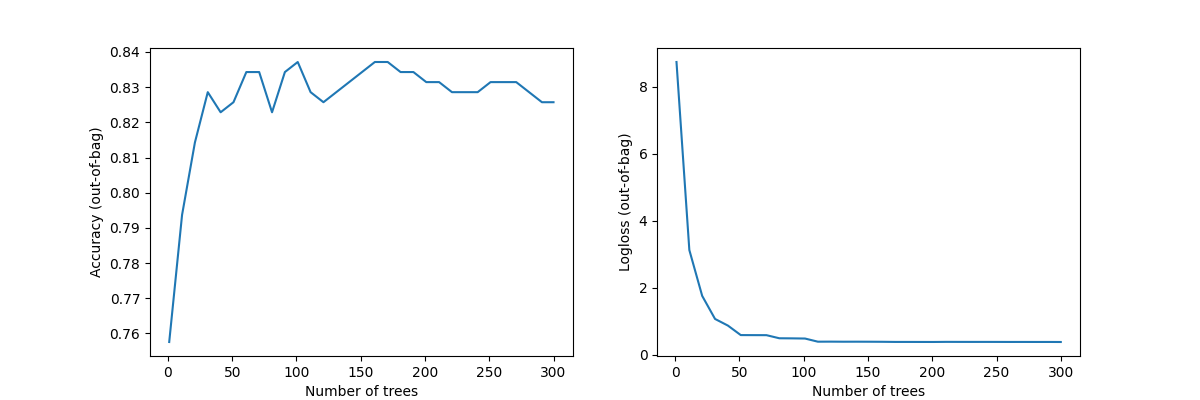
\includegraphics[width=\textwidth]{images/defaultModelAcc.png}
    \caption{Random Forest (Default Model)}
    \label{fig:1}
\end{figure}
\begin{figure}[H]
    \centering
    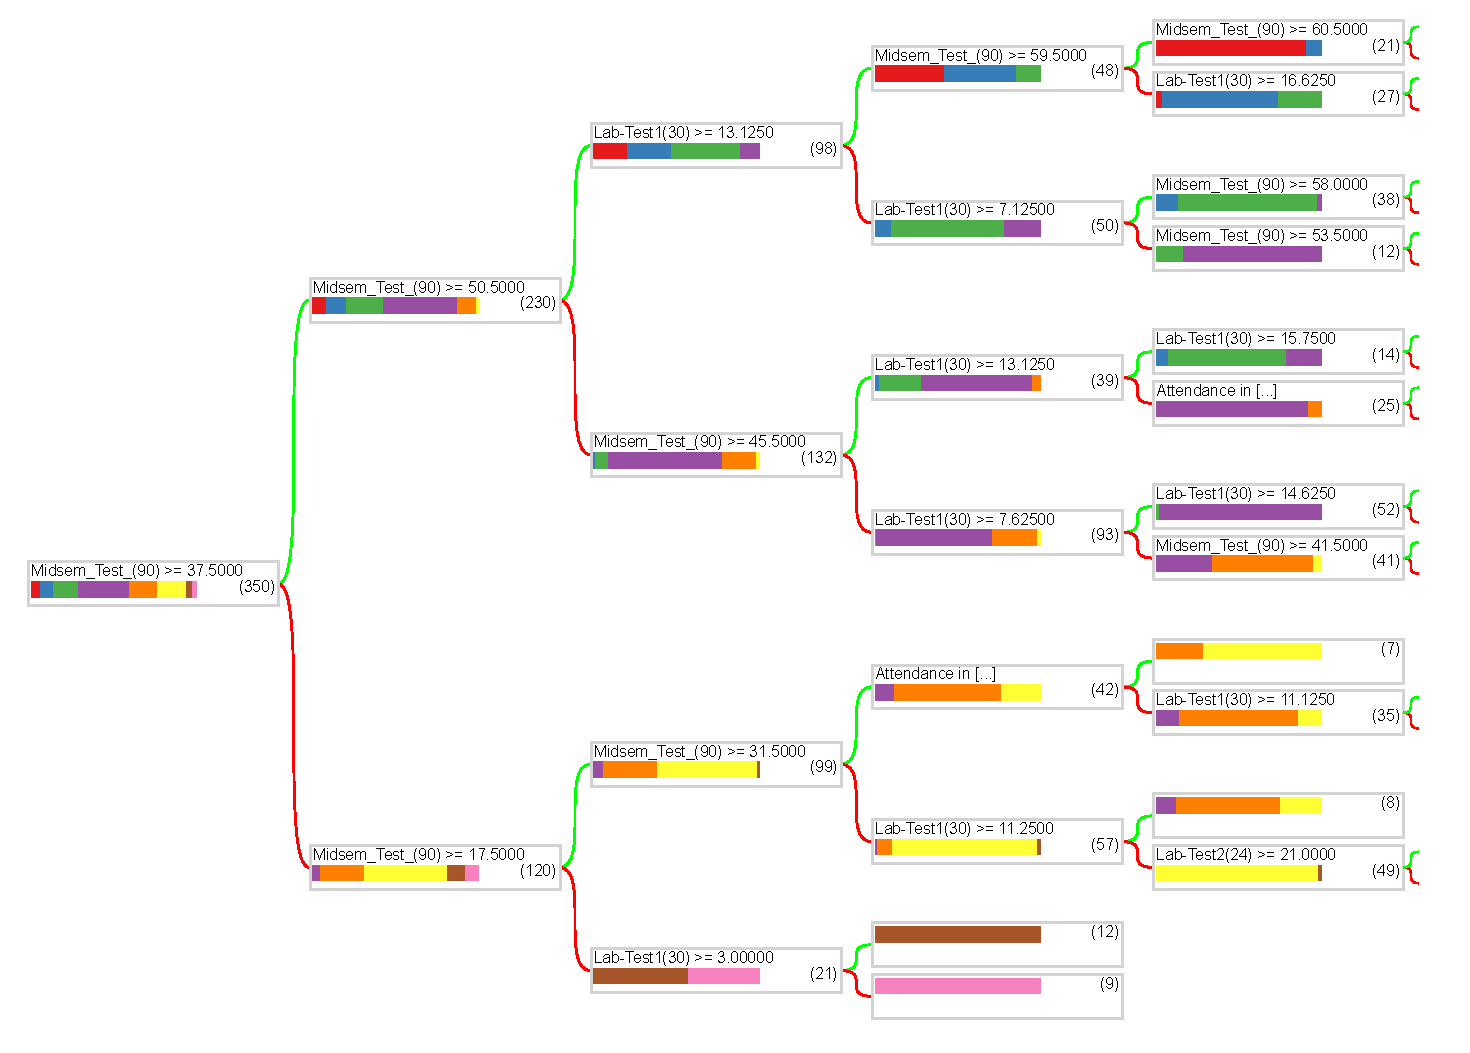
\includegraphics[width=\textwidth]{images/defModel.pdf}
    \caption{Random Forest (Default Model)}
    \label{fig:5}
\end{figure}


\subsection{Random Forest (Tuned Model)}
Accuracy: 87.33\% \\
Number of trees: 300 \\
The drop in accuracy could be due to overfitting. \\
% Hyperparameters: \{\} \\
\begin{figure}[h]
    \centering
    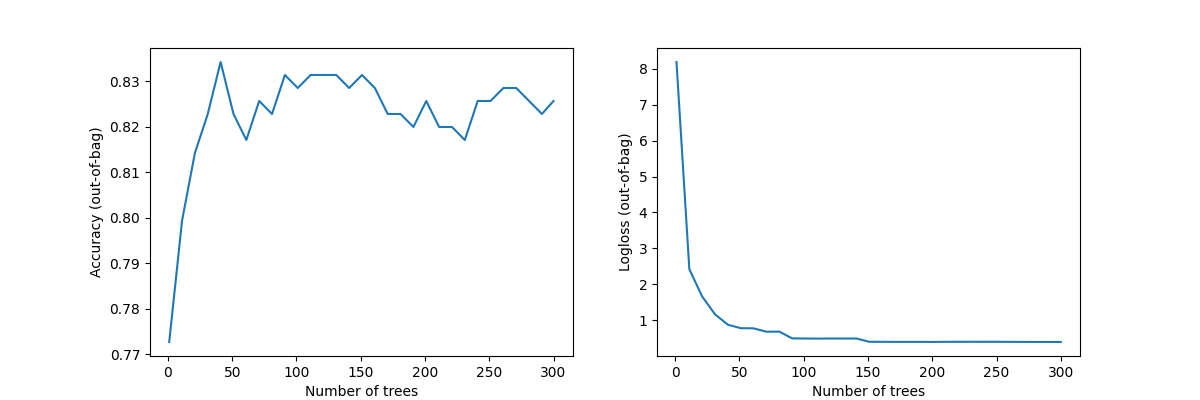
\includegraphics[width=\textwidth]{images/tunedModelAcc.png}
    \caption{Random Forest (Improved Model)}
    \label{fig:2}
\end{figure}
\begin{figure}[H]
    \centering
    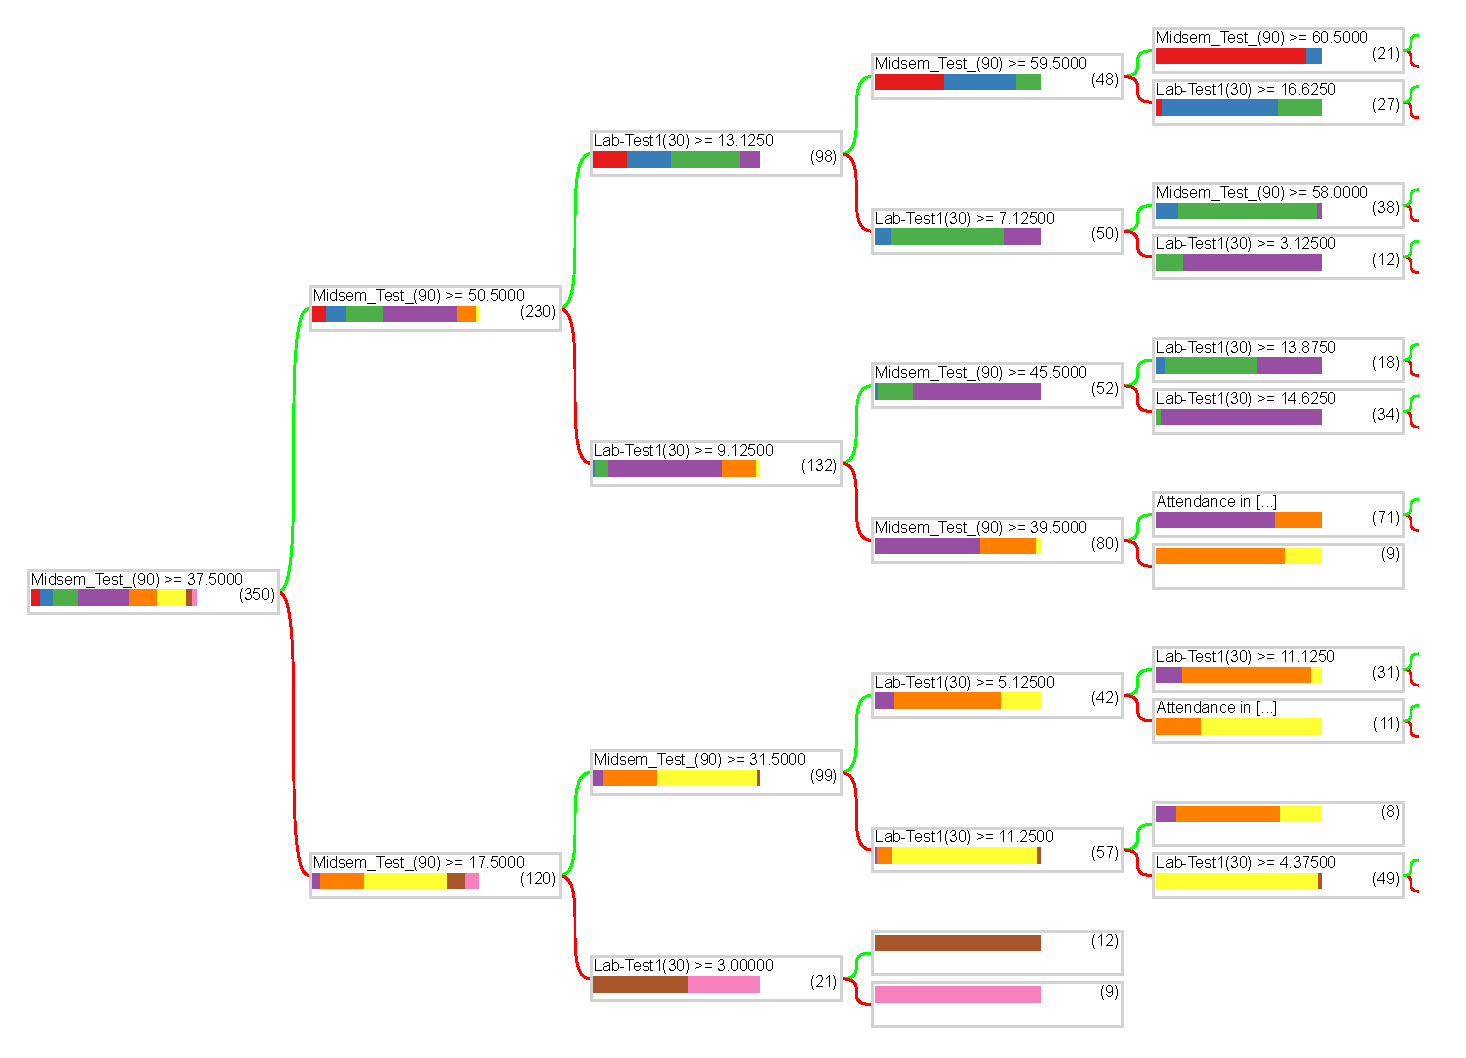
\includegraphics[width=\textwidth]{images/imprModel.pdf}
    \caption{Random Forest (Improved Model)}
    \label{fig:6}
\end{figure}

\subsection{Random Forest (Reduced Model)}
Accuracy: 88.00\% \\
Number of trees: 30 \\
% Hyperparameters: \{\} \\
Restricting the number of trees to 30 gives a much better accuracy, since on 300 trees model could be overfitting due to limited sample size of data.
\begin{figure}[h]
    \centering
    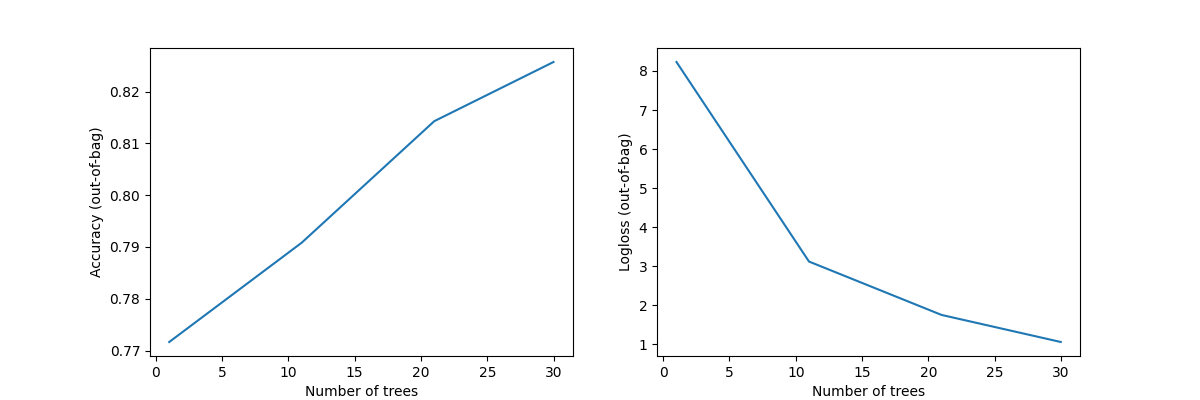
\includegraphics[width=\textwidth]{images/reducedModelAcc.png}
    \caption{Random Forest (Reduced Model)}
    \label{fig:3}
\end{figure}

\savegeometry{before_landscape}
\begin{landscapes}
    \centering
  \includesvg[width=\textwidth]{tree.svg}
  First tree in the trained Random Forest
\end{landscapes}
\loadgeometry{before_landscape}

\begin{figure}[H]
    \centering
    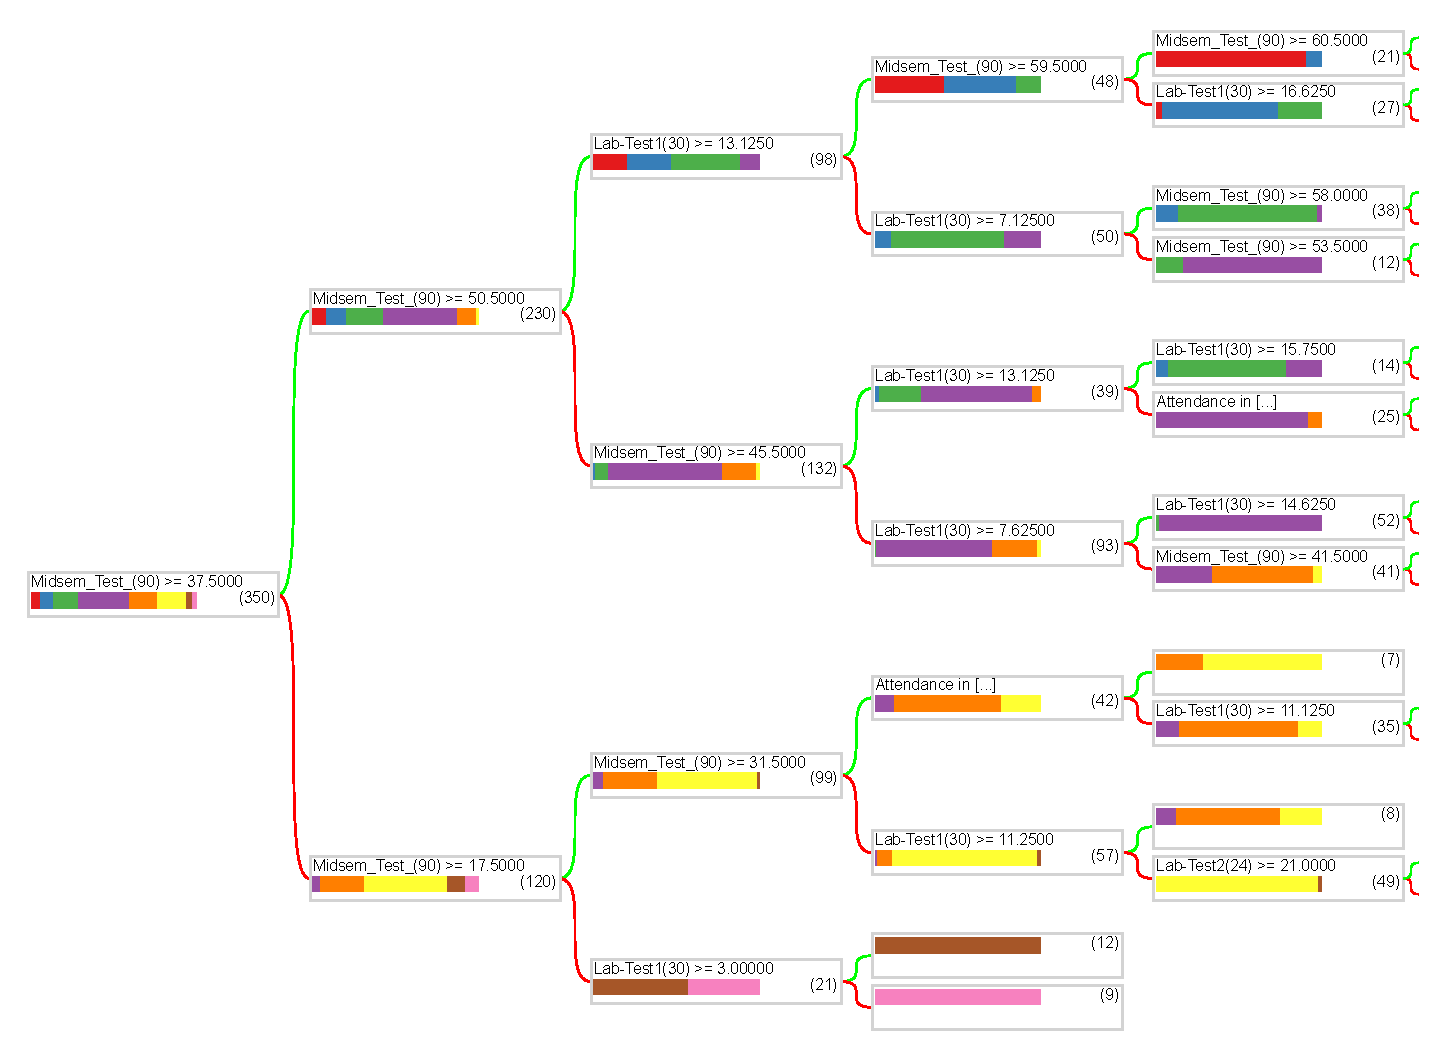
\includegraphics[width=\textwidth]{images/redModel.pdf}
    \caption{Random Forest (Reduced Model)}
    \label{fig:7}
\end{figure}

\subsection{Random Forest (Without encoding)}
Accuracy: 87.33\% \\
Though we expect a decrease in accuracy, due to randomness and limited data, there is no significant change. \\
\subsection{Gradient Boosted Decision Trees}
Accuracy: 87.33\% \\
Number of trees: 30 \\
%Hyperparameters: \{\} \\
\begin{figure}[H]
    \centering
    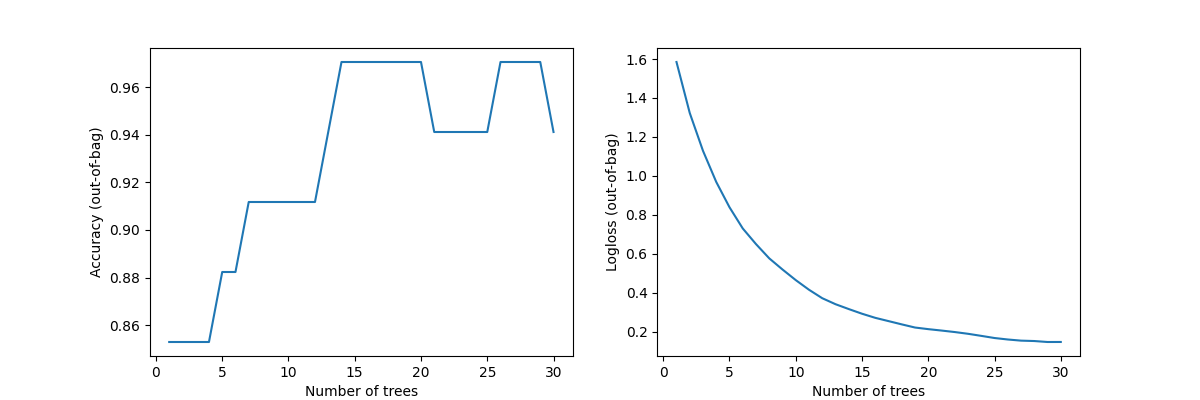
\includegraphics[width=\textwidth]{images/gbdtAcc.png}
    \caption{Gradient Boosted Decision Trees}
    \label{fig:4}
\end{figure}
\begin{figure}[H]
    \centering
    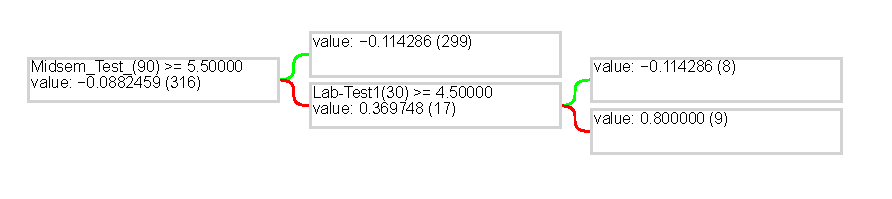
\includegraphics[width=\textwidth]{images/gbdt.pdf}
    \caption{Gradient Boosted Decision Trees}
    \label{fig:8}
\end{figure}

\subsection{Analysis of Parameters in Random Forests}
Train Accuracy = 95.43\% \\
Test Accuracy = 88\% \\
As expected train accuracy is much higher than test accuracy.
\subsubsection*{Number of Trees}
\begin{figure}[H]
    \centering
    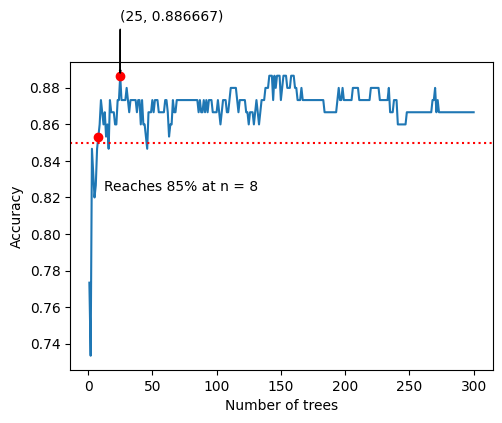
\includegraphics[width=0.45\textwidth]{images/notrees.png}
    \caption{Accuracy with number of trees}
    \label{fig:9}
\end{figure}
\subsubsection*{Maximum Depth}
\begin{figure}[H]
    \centering
    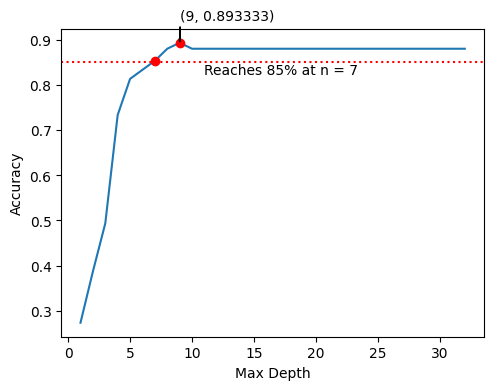
\includegraphics[width=0.45\textwidth]{images/deptrees.png}
    \caption{Accuracy with maximum depth, with n = 30}
    \label{fig:10}
\end{figure}
%\subsection{Normalisation of attributes}%
 

\bigskip


\section{Glossary}
$$\text{Accuracy} = \frac{TP+TN}{TP+FP+TN+FN}$$
$$\text{Log Loss} = -\frac{1}{n}\sum{(y \times \log{(p)})}$$

%\par \finalresult{Therefore, cats are equal to infinity.}
\end{document}
